% ---
\documentclass{article}


% Packages
% ---
\usepackage{amsmath,amssymb,amsthm} 	% Advanced math typesetting
% \usepackage[utf8]{inputenc} 	% Unicode support (Umlauts etc.)
\usepackage[USenglish]{babel} 	% Change hyphenation rules
\usepackage{hyperref} 				% Add a link to your document
\usepackage{graphicx}				% Add pictures to your document
\graphicspath{ {./images/} }	% image directory
\usepackage{listings} 				% Source code formatting and highlighting
\lstset{basicstyle=\ttfamily}		%Typewriter font for code writing
\usepackage{geometry}
\geometry{margin=1in}
\usepackage{enumitem}
\usepackage{float}
%\floatstyle{boxed}
\restylefloat{figure}
\usepackage{mathabx}
\usepackage{fancyhdr}

\pagestyle{fancy}
\fancyhf{}
\lhead{\bf CPSC 340 \\ Week 1 }
\rhead{\bf Jeremi Do Dinh \\ 61985628}
\rfoot{Page \thepage}



\usepackage{tikz}						% Graph drawing tools
\usetikzlibrary {positioning}

\usepackage{breqn}
\usepackage{multicol} 				% Multiple column functionality
\usepackage{blindtext}


\begin{document}
	
\noindent \url{https://www.cs.ubc.ca/~fwood/CS340/}

\section*{Lecture II}
Lecture roughly follows: \url{http://www-users.cs.umn.edu/~kumar/dmbook/dmslides/chap2_data.pdf} \\
Slides: \url{https://www.cs.ubc.ca/~fwood/CS340/lectures/L2.pdf}\\

\subsection*{Data Mining: Some Typical Steps}

\begin{enumerate}
	\item Learn about the application.
	\item Identify data mining task.
	\item Collect data.
	\item Clean and preprocess the data.
	\item Transform data or select useful subsets.
\item Choose data mining algorithm.
\item Data mining!
\item Evaluate, visualize, and interpret results.
\item Use results for profit or other goals.\\
	(often, you’ll go through cycles of the above)
\end{enumerate}

\subsubsection*{What is data?}
We'll define data as a collection of {\bf examples}, and their {\bf features} 

\subsubsection*{Types of data}
\begin{itemize}
	\item Categorical features come from an unordered set
	\begin{itemize}
		\item Binary: Job done or not?
		\item Nominal: city
	\end{itemize}
	\item Numerical features come from an ordered sets
	\begin{itemize}
		\item Discrete counts: age
		\item Ordinal: rating
		\item Continuous/real-values: height
	\end{itemize}
\end{itemize}

\subsection*{Converting to numerical features}
It is very often more desirable to have real-values example representation.
\begin{figure}[H]
	\centering
	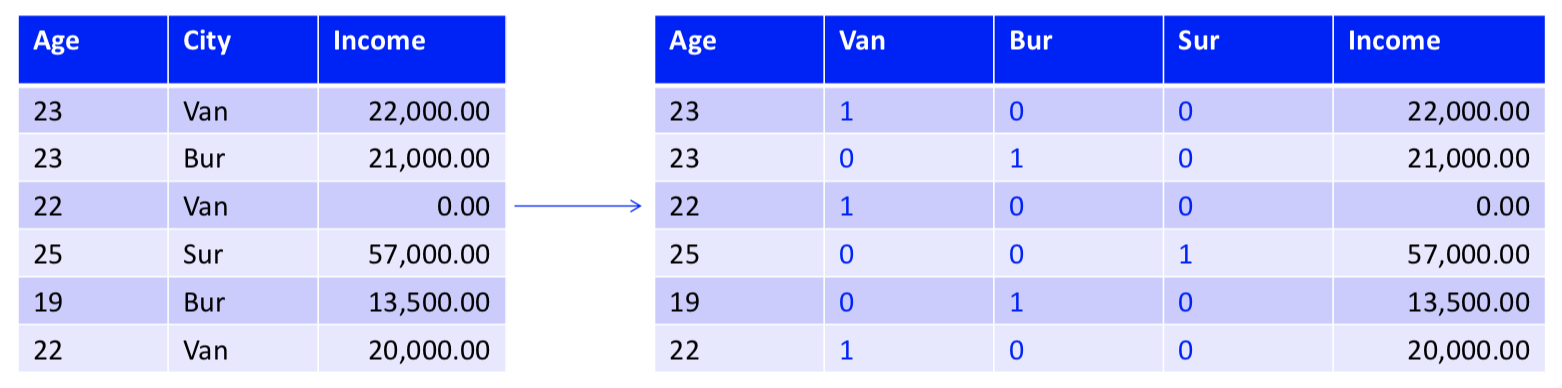
\includegraphics[width = 6in]{Pic1}
\end{figure}
\noindent This is called {\bf 1 of k encoding}, and we can now interpret examples as points in space (E.g., first example is at (23,1,0,0,22000))
\subsubsection*{Approximating Text with Numerical Features}
\begin{figure}[H]
	\centering
	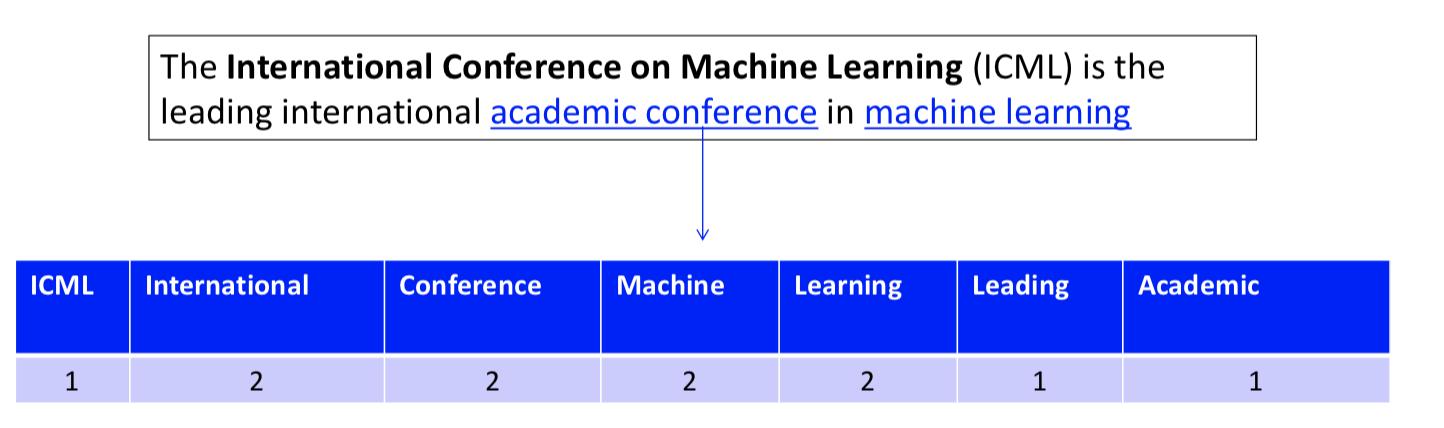
\includegraphics[width = 4in]{Pic2}
\end{figure}

\subsubsection*{Approximating Images and Graphs}
\begin{figure}[H]
	\centering
	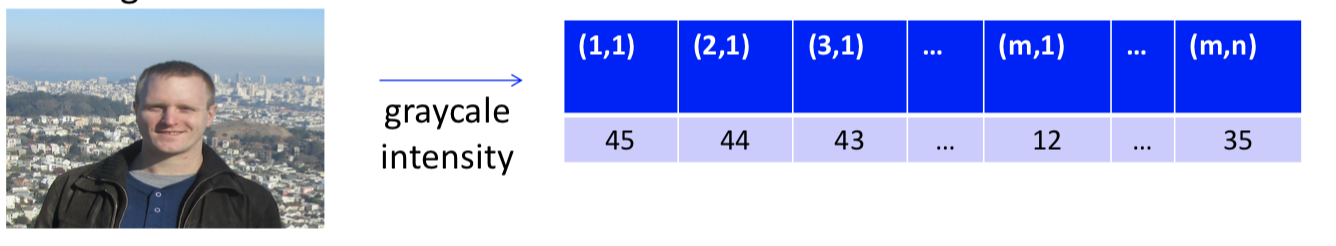
\includegraphics[width = 5in]{Pic3}
\end{figure}
\begin{figure}[H]
	\centering
	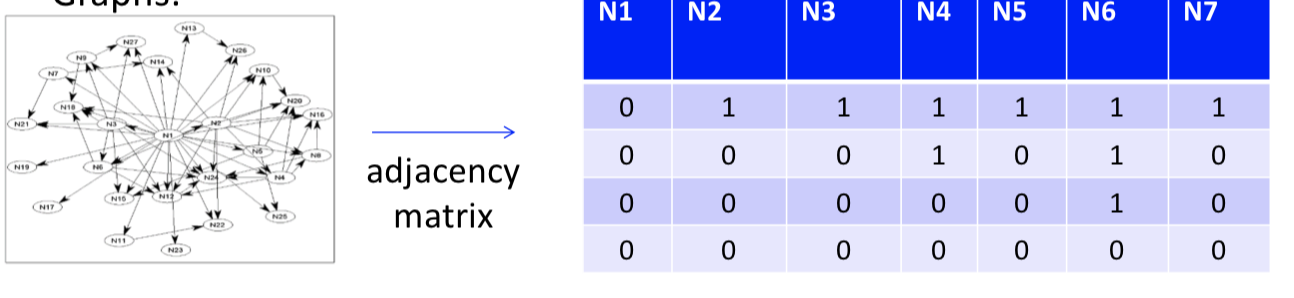
\includegraphics[width = 5in]{Pic4}
\end{figure}

\subsection*{Data Cleaning}
ML+DM typically assume ‘clean’ data. Ways that data might not be ‘clean’ : 
\begin{itemize}
	\item Noise (e.g., distortion on phone).
	\item Outliers (e.g., data entry or instrument error).
	\item Missing values (no value available or not applicable)
	\item Duplicated data (repetitions, or different storage formats).
\end{itemize}
Any of these can lead to problems in analyses
\begin{itemize}
	\item Want to fix these issues, if possible.
	\item Some ML methods are robust to these.
	\item Often, ML is the best way to detect/fix these.
\end{itemize}


\end{document}